% JuliaCon proceedings template
%\documentclass[]{article}
\documentclass{juliacon}
\setcounter{page}{1}

%\usepackage[utf8]{inputenc}

\usepackage{graphicx}
\usepackage{subcaption}
%\usepackage[left=1.00in, right=1.00in, top=1.00in, bottom=1.00in]{geometry}

\usepackage{dirtytalk}
\usepackage[normalem]{ulem}
\usepackage{tikz-cd}
\usepackage{units}
\usepackage{algorithm}
\usepackage{algpseudocode}
\usepackage{alltt}
\usepackage{mathrsfs}
\usepackage{amssymb}
\usepackage{amsmath}
\DeclareMathOperator\cis{cis}
\newenvironment{rcases}
  {\left.\begin{aligned}}
  {\end{aligned}\right\rbrace}
\newenvironment{acases}
  {\left.\begin{aligned}}
  {\end{aligned}\right}

% (font shortcuts)
\usepackage{amsfonts}
\newcommand{\mb}[1]{\mathbb{#1}}
\newcommand{\mc}[1]{\mathcal{#1}}
\newcommand{\ms}[1]{\mathscr{#1}}
\newcommand{\mf}[1]{\frak{#1}}

% (arrow shortcuts)
\newcommand{\ra}{\rightarrow}
\newcommand{\lra}{\longrightarrow}
\newcommand{\la}{\leftarrow}
\newcommand{\lla}{\longleftarrow}
\newcommand{\Ra}{\Rightarrow}
\newcommand{\Lra}{\Longrightarrow}
\newcommand{\La}{\Leftarrow}
\newcommand{\Lla}{\Longleftarrow}
\newcommand{\lr}{\leftrightarrow}
\newcommand{\llr}{\longleftrightarrow}
\newcommand{\Lr}{\Leftrightarrow}
\newcommand{\Llr}{\Longleftrightarrow}
\newcommand{\ua}{\uparrow}
\newcommand{\da}{\downarrow}
\newcommand{\Ua}{\Uparrow}
\newcommand{\Da}{\Downarrow}

% (match parenthesis)
\newcommand{\mlr}[1]{\left|#1\right|}
\newcommand{\plr}[1]{\left(#1\right)}
\newcommand{\blr}[1]{\left[#1\right]}
\newcommand{\nlr}[1]{\mlr{\mlr{#1}}}
\newcommand{\nlrp}[2]{\nlr{#1}_{#2}}

% (exponent shortcuts)
\newcommand{\inv}{^{-1}}
\newcommand{\nrt}[2]{\sqrt[\leftroot{-2}\uproot{2}#1]{#2}}

% (annotation shortcuts)
\newcommand{\conj}[1]{\overline{#1}}
\newcommand{\ol}[1]{\overline{#1}}
\newcommand{\ul}[1]{\underline{#1}}
\newcommand{\os}[2]{\overset{#1}{#2}}
\newcommand{\us}[2]{\underset{#1}{#2}}
\newcommand{\ob}[2]{\overbrace{#2}^{#1}}
\newcommand{\ub}[2]{\underbrace{#2}_{#1}}
\newcommand{\bs}{\backslash}
\newcommand{\ds}{\displaystyle}

% (set builder)
\newcommand{\set}[1]{\left\{ #1 \right\}}
\newcommand{\setc}[2]{\left\{ #1 : #2 \right\}}
\newcommand{\setm}[2]{\left\{ #1 \, \middle| \, #2 \right\}}
\newcommand{\Cp}[2]{C^{#1}(#2)}
\newcommand{\Cb}[3]{C^{#1}{[}#2,#3{]}}
\newcommand{\Cpb}[3]{C^{#1}({[}#2,#3{]})}
%\newcommand{\C}[3]{\Cb{#1}{#2}{#3}}

% (group generator)
\newcommand{\gen}[1]{\left\langle #1 \right\rangle}

% (functions)
\newcommand{\im}[1]{\text{im}(#1)}
\newcommand{\range}[1]{\text{range}(#1)}
\newcommand{\domain}[1]{\text{domain}(#1)}
\newcommand{\dist}[1]{(#1)}
\newcommand{\sgn}{\text{sgn}}

% (sums)
\newcommand{\lset}[2]{#2_1,\dots,#2_{#1}}
\newcommand{\lsum}[2]{#2_1+\dots+#2_{#1}}
\newcommand{\norm}[3]{|#2_1|^{#1}+\dots+|#2_{#3}|^{#1}}
\newcommand{\norms}[4]{\sum_{#2=1}^{#4}|#3_{#2}|^{#1}}
\newcommand{\lc}[3]{#2_1#3_1+\dots+#2_{#1}#3_{#1}}
\newcommand{\lcs}[4]{\sum_{#4=1}^{#1}#2_{#4}#3_{#4}}

% (Linear Algebra)
\newcommand{\mat}[1]{\begin{bmatrix}#1\end{bmatrix}}
\newcommand{\pmat}[1]{\begin{pmatrix}#1\end{pmatrix}}
%\newcommand{\dim}[1]{\text{dim}(#1)}
\newcommand{\rnk}[1]{\text{rank}(#1)}
\newcommand{\nul}[1]{\text{nul}(#1)}
\newcommand{\spn}[1]{\text{span}\,#1}
\newcommand{\col}[1]{\text{col}(#1)}
%\newcommand{\ker}[1]{\text{ker}(#1)}
\newcommand{\row}[1]{\text{row}(#1)}
\newcommand{\area}[1]{\text{area}(#1)}
\newcommand{\nullity}[1]{\text{nullity}(#1)}
\newcommand{\proj}[2]{\text{proj}_{#1}\left(#2\right)}
\newcommand{\diam}[1]{\text{diam}\,#1}

% (Vectors common)
\newcommand{\myvec}[1]{\vec{#1}}
\newcommand{\va}{\myvec{a}}
\newcommand{\vb}{\myvec{b}}
\newcommand{\vc}{\myvec{c}}
\newcommand{\vd}{\myvec{d}}
\newcommand{\ve}{\myvec{e}}
\newcommand{\vf}{\myvec{f}}
\newcommand{\vg}{\myvec{g}}
\newcommand{\vh}{\myvec{h}}
\newcommand{\vi}{\myvec{i}}
\newcommand{\vj}{\myvec{j}}
\newcommand{\vk}{\myvec{k}}
\newcommand{\vl}{\myvec{l}}
\newcommand{\vm}{\myvec{m}}
\newcommand{\vn}{\myvec{n}}
\newcommand{\vo}{\myvec{o}}
\newcommand{\vp}{\myvec{p}}
\newcommand{\vq}{\myvec{q}}
\newcommand{\vr}{\myvec{r}}
\newcommand{\vs}{\myvec{s}}
\newcommand{\vt}{\myvec{t}}
\newcommand{\vu}{\myvec{u}}
\newcommand{\vv}{\myvec{v}}
\newcommand{\vw}{\myvec{w}}
\newcommand{\vx}{\myvec{x}}
\newcommand{\vy}{\myvec{y}}
\newcommand{\vz}{\myvec{z}}
\newcommand{\vzero}{\myvec{0}}


% Theorems and Propositions
%\usepackage{amsthm}
%\newtheorem{theorem}{Theorem}
%\newtheorem{proposition}{Proposition}

%\theoremstyle{definition}
%\newtheorem{definition}{Definition}

%\theoremstyle{remark}
%\newtheorem*{remark}{Remark}
%\newtheorem{example}{Example}
%\newtheorem*{recall}{Recall}
%\newtheorem*{remark}{Note}
%\newtheorem*{observe}{Observe}
%\newtheorem*{question}{\underline{Question}}
%\newtheorem*{fact}{Fact}
%\newtheorem{corollary}{Corollary}
%\newtheorem*{lemma}{Lemma}
%\newtheorem{xca}{Exercise}

\usepackage{unicode-math}
\setmonofont[Scale=MatchLowercase]{DejaVu Sans Mono}
\usepackage{scalerel}
\DeclareMathOperator*{\bigboxtimes}{\scalerel*{\boxtimes}{\bigodot}}
\DeclareMathOperator*{\bigominus}{\scalerel*{\ominus}{\bigodot}}
\DeclareMathOperator*{\obackslash}{\text{\reflectbox{$\oslash$}}}

\author{Michael Reed (Crucial Flow Research)}
\title{Differential geometric algebra with Leibniz and Grassmann}
\date{July 25th, 2019}

\begin{document}

%% **************GENERATED FILE, DO NOT EDIT**************

\title{Differential geometric algebra using Leibniz, Grassmann}

\author[1]{Michael Reed}
\affil[1]{Crucial Flow Research, Computational Meta-Linguist}

\keywords{Julia, Geometric Algebra, Differential Geometry, Multiple Dispatch, Metaprogramming}



\maketitle
\begin{figure}[ht]
%\centerline{\includegraphics[width=4cm]{img/grassmann.png}}
\centerline{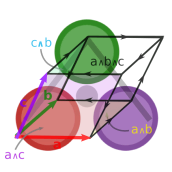
\includegraphics[width=4cm]{../docs/src/assets/logo.png}}
\caption*{github.com/chakravala/Grassmann.jl}
\end{figure}
\begin{abstract}
	The \textit{Grassmann.jl}
	package provides tools for computations based on multi-linear algebra and spin groups using the extended geometric algebra known as Leibniz-Grassmann-Clifford-Hestenes algebra.
	Combinatorial products include
	exterior, regressive, inner, and geometric; along with the Hodge star, adjoint, reversal, and boundary operators.
	The kernelized operations are built up from composite sparse tensor products and Hodge duality, with high dimensional support for up to 62 indices using staged caching and precompilation. Code generation enables concise yet highly extensible definitions.
	\textit{DirectSum.jl}
	multivector parametric type polymorphism is based on tangent vector spaces and conformal projective geometry.
	Additionally, the universal interoperability between different sub-algebras is enabled by \textit{AbstractTensors.jl},
	on which the type system is built.
	%\headingtable
\end{abstract}
\begin{itemize}
	\item \textbf{DirectSum.jl}: Abstract tangent bundle vector space types (unions, intersections, sums, etc.)
	\item \textbf{AbstractTensors.jl}: Tensor algebra abstract type interoperability with vector bundle parameter
	\item \textbf{Grassmann.jl}: $\langle$Leibniz+Grassmann-Clifford-Hestenes$\rangle$ differential geometric algebra of multivector forms
	\item \textbf{Leibniz.jl}: Derivation operator algebras for tensor fields
	\item \textbf{Reduce.jl}: Symbolic parser generator for Julia expressions using REDUCE algebra term rewriter
\end{itemize}
Mathematical foundations and some of the nuances in the definitions specific to the \textit{Grassmann.jl} implementation are concisely described, along with the accompanying support packages that provide an extensible platform for computing with geometric algebra at high dimensions.
The design is based on the \verb`TensorAlgebra` abstract type interoperability from \textit{AbstractTensors.jl} with a \verb`VectorBundle` type parameter from \textit{DirectSum.jl}. Abstract vector space type operations happen at compile-time, resulting in a differential conformal geometric algebra of hyper-dual multivector forms.

The nature of the geometric algebra code generation enables one to easily extend the abstract product operations to any specific number field type (including differential operators with \textit{Leibniz.jl} or symbolic coefficients with \textit{Reduce.jl}), by making use of Julia's type system. Mixed tensor products with their coefficients are constructed from these operations to work with bivector elements of Lie groups \cite{hestenes}\cite{shahshahani}.

\section{Direct sum parametric type polymorphism}

The \textit{DirectSum.jl} package is a work in progress providing the necessary tools to work with an arbitrary \verb`Manifold` specified by an encoding. Due to the parametric type system for the generating \verb`VectorBundle`, the Julia compiler can fully pre-allocate and often cache values efficiently ahead of run-time.
Although intended for use with the \textit{Grassmann.jl} package, \verb`DirectSum` can be used independently.

\begin{definition}[Vector bundle of submanifolds]
	Let $M = T^\mu V\in\text{Vect}_{\mb K}$ be a \verb`VectorBundle<:Manifold` of rank $n$,
	\begin{align*}
		T^\mu V &= (n,\mb P,g,\nu,\mu), & \mb P &\subseteq\gen{v_\infty,v_\emptyset}, & g &:V\times V\ra\mb K
	\end{align*}
	The type \verb+VectorBundle{n,+$\mb P$\verb+,g,+$\nu,\mu$\verb+}+ uses \textit{byte-encoded} data available at pre-compilation, where
	$\mb P$ specifies the basis for up and down projection,
	$g$ is a bilinear form that specifies the metric of the space,
	and $\mu$ is an integer specifying the order of the tangent bundle (i.e. multiplicity limit of Leibniz-Taylor monomials). Lastly, $\nu$ is the number of tangent variables.
\end{definition}
The dual space functor $(\cdot)':\text{Vect}_{\mb K}^\text{op}\ra\text{Vect}_{\mb K}$
is an involution which toggles a dual vector space with inverted signature with property $V' = \text{Hom}(V,\mb K)$ and having \verb`Basis` generators
$$\gen{v_1,\dots,v_{n-\nu},\partial_1,\dots,\partial_\nu}=M\leftrightarrow M' = \gen{w_1,\dots,w_{n-\nu},\epsilon_1,\dots,\epsilon_\nu}$$
where $v_i,w_i$ are a basis for the vectors and covectors, while $\partial_j,\epsilon_j$ are a basis for differential operators and tensor fields.

The direct sum operator \verb`⊕` can be used to join spaces (alternatively \verb`+`).
The direct sum of a \verb`VectorBundle` and its dual \verb`V⊕V'` represents the full mother space \verb`V*`.
In addition to the direct-sum operation, several other operations exist, such as $\cup,\cap,\subseteq,\supseteq$ for set operations.
Due to the design of the \verb`VectorBundle` dispatch, these operations enable code optimizations at compile-time provided by the bit parameters.
$$ \bigcup T^{\mu_i}V_i = \plr{|\mb P|+\max\set{n_i-|\mb P_i|}_i,\, \bigcup \mb P_i,\, \cup g_i,\, \max\set{\mu_i}_i} $$
$$ \bigoplus T^{\mu_i}V_i = \plr{\mlr{\mb P}+\sum (n_i-|\mb P_i|),\, \bigcup \mb P_i,\, \oplus_i g_i,\,\max\set{\mu_i}_i} $$
These are roughly the formulas used for those operations.
%\end{definition}
\begin{remark}
	Although some type operations like $\bigcup$ and $\bigoplus$ are similar and sometimes result in equal values, the union and sum are entirely different operations in general.
\end{remark}

Calling manifolds with sets of indices constructs the subspace representations.
Given \verb`M(s::Int...)` one can encode \verb+SubManifold{+$|s|,M,s$\verb+}+ with induced orthogonal space $Z$:
$$T^eV \subset T^\mu W \iff \exists Z\in\text{Vect}_{\mb K}(T^e(V\oplus Z) = T^{e\leq \mu}W,\,V\perp Z),$$
such that computing unions of submanifolds is done by inspecting the parameter $s\in V\subseteq W$ and $s\notin Z$. Operations on \verb`Manifold` types is automatically handled at compile time.

The metric signature of the \verb+Basis{V,1}+ elements of a vector space \verb+V+ can be specified with the \verb+V"..."+ constructor by using \verb-+- and \verb+-+ to specify whether the \verb+Basis{V,1}+ element of the corresponding index squares to \verb`+1` or \verb`-1`.
For example, \verb`S"+++"` constructs a positive definite 3-dimensional \verb`VectorBundle`.
It is also possible to specify an arbitrary \verb`DiagonalForm` having numerical values for the basis with degenracy \verb`D"1,1,1,0"`, although the $\pm$ format has a more compact representation.
Further development will result in more metric types.

Declaring an additional plane at infinity is done by specifying it in the string constructor with \verb`∞` at the first index (i.e. Riemann sphere \verb`S"∞+++"`). The hyperbolic geometry can be declared by \verb`∅` subsequently (i.e. Minkowski spacetime \verb`S"∅+++"`). 
Additionally, the \textit{null-basis} based on the projective split for confromal geometric algebra would be specified with \verb`∞∅` initially (i.e. 5D CGA \verb`S"∞∅+++"`). These two declared basis elements are interpreted in the type system. %such that they are automatically selected for up and down projection.
%propagate under transformations when combining mixed index sets (provided the \verb`Signature` is compatible).

The \verb`tangent(V,`$\mu$\verb`,`$\nu$\verb`)` map can be used to specify $\mu$ and $\nu$.

\section{Tensor basis equivalence classes}% of Leibniz and Grassmann}

The \verb`AbstractTensors` package is intended for universal interoperability of the abstract \verb`TensorAlgebra` type system.
All \verb`TensorAlgebra{V}` subtypes have type parameter \verb`V`, used to store a \verb`VectorBundle` value obtained from \textit{DirectSum.jl}.
By itself, this package does not impose any specifications or structure on the \verb`TensorAlgebra{V}` subtypes and elements, aside from requiring $V$ to be a \verb`VectorBundle`.
Hence all tensor types share a common underlying \verb`VectorBundle` structure.
The macro \verb`@basis V` declares a local basis in Julia.

\begin{definition}
	Let $V\in\text{Vect}_{\mb k}$ be a \verb`VectorBundle` with dual space $V'$ and the basis elements $w_k:V\ra\mb K$, then for all $x\in V,c\in\mb K$ the properties $(w_i+w_j)(x) = w_i(x)+w_j(x)$ and $(cw_k)(x) = cw_k(x)$ hold.
	An element of a mixed-symmetry \verb`TensorAlgebra{V}` is a multilinear mapping that is formally constructed by taking the tensor products of linear and multilinear maps,
	$(\bigotimes_k \omega_k)(v_1,\dots,v_{\sum_k p_k}) = \prod_k \omega_k(v_1,\dots,v_{p_k})$.
\end{definition}
\begin{definition}[Mixed-symmetry basis]
	Combining the linear basis generating elements with each other using the multilinear tensor product yields a graded (decomposable) tensor \verb`Basis` $\langle w_{p_1}\otimes\dots\otimes w_{p_k}\rangle_k$, where \verb`grade` $k$ is determined by the number of $w_i$ basis elements in its tensor product decomposition.
	The algebra partitions into symmetric and anti-symmetric tensor equivalence classes.
	For any pair, %of tensors, either
	\begin{align*}
		&\us{\text{anti-symmetric}}{\omega\otimes\eta = -\eta\otimes\omega} & \text{or} &  &\us{\text{symmetric}}{\omega\otimes\eta = \eta\otimes\omega}.
	\end{align*}
	Typically the $k$ in a product $\plr{\partial_{p_1}\otimes\cdots\otimes\partial_{p_k}}^{(k)}$ is referred to as the \verb`order` of the element if it is fully symmetric, which is overall tracked separately from the \verb`grade` such that $\partial_k\gen{w_j}_r = \gen{\partial_kw_j}_r$ and $(\partial_k)^{(r)}\omega_j = (\partial_kw_j)^{(r)}$.
	Hence, there is a partitioning into \verb`even` grade components $\omega_+$ and \verb`odd` grade components $\omega_-$ such that $\omega_++\omega_-=\omega$.
\end{definition}
\begin{remark}
	Observe that the anti-symmetric property implies that $\omega\otimes\omega=0$, while the symmetric property neither implies nor denies such a property.
	Grassmann remarked \cite{grassmann-2} in 1862 that the symmetric algebra of functions is by far more complicated than his anti-symmetric exterior algebra.
	The first part of the book focused on anti-symmetric exterior algebra, while the more complex symmetric function algebra of Leibniz was subject of the second multivariable part of the book.
	Elements $\omega_k$ in the space $\Lambda V$ of anti-symmetric algebra are often studied as unit quantum state vectors in a unitary probability space, where $\sum_k\omega_k\neq\bigotimes_k\omega_k$ is entanglement.
\end{remark}
\begin{definition}
	The Grassmann anti-symmetric exterior basis is denoted by $v_{i_1\dots i_g}\in\Lambda_gV$ with its dual $w^{i_1\cdots i_g}\in\Lambda^gV$, while the Leibniz symmetric basis will be $\partial_{i_1}^{\mu_1}\dots\partial_{i_g}^{\mu_g}\in L_gV$ with $\epsilon_{i_1}^{\mu_1}\dots\epsilon_{i_g}^{\mu_g}\in L^gV$ dual elements. Let $\Lambda V = \bigoplus \Lambda^g V$.
\end{definition}
A higher-order tensor element is an oriented-multi-set $X$ %\in\text{OMSet}$
such that $w_X = \bigotimes_k w_{i_k}^{\otimes\mu_k}$ with $X = \plr{(i_1,\mu_1),\dots,(i_g,\mu_g)}$ and $|X|=\sum_k\mu_k$ is \verb`grade`,$\,$ \verb`order`.
%There are two orientations and higher multiplicities result in zero for anti-symmetric tensors denoted by indices $\Lambda X\subseteq\Lambda V$, so the only interesting multiplicity is $\mu_k\equiv 1$.
Anti-symmetric indices $\Lambda X\subseteq\Lambda V$ have two orientations and higher multiplicities are degenerate, hence the only relevant multiplicity is $\mu_k\equiv 1$.
%Symmetric tensors have an ambiguous multiplicity of nilpotence; decide that $\epsilon_k^{\mu+1}=0$, so $\mu_k\leq\mu$ can be non-trivial, negative, or unbounded.
The Leibniz-Taylor algebra \cite{taylor-algebra} is a quotient polynomial ring $LV\cong R[x_1,\dots,x_n]/\{\prod_{k=1}^{\mu+1} x_{p_k}\}$, so that $\epsilon_k^{\mu+1}=0$. % is $\mu$ truncated % (e.g. Jacobian and Hessian).

The Grassmann \verb`Basis` elements $v_k\in\Lambda_1V$ and $w^k\in\Lambda^1V$ are linearly independent vector and covector elements of $V$, while the Leibniz \verb`Operator` elements $\partial_k\in L_1V$ are partial tangent derivations and $\epsilon_k(x)\in L^1V$ are dependent functions of the \verb`tangent` manifold. 
Higher \verb`grade` elements of $\Lambda V$ correspond to \verb`SubManifold` spaces, while higher \verb`order` function elements of $LV$ become homogenous polynomials and Taylor series.

%Grassmann's exterior algebra is fundamentally simpler in structure than the symmetric generated algebra,
Grassmann's exterior algebra doesn't invoke the properties of multi-sets, as it is related to the algebra of oriented sets; while the Leibniz symmetric algebra is that of unoriented multi-sets.
Combined, the mixed-symmetry algebra yield a multi-linear propositional lattice.
The formal sum of equal \verb`grade` elements is an oriented \verb`Chain` and with mixed \verb`grade` it is a \verb`MultiVector` simplicial complex.
Thus, various standard operations on the oriented multi-sets are possible including $\cup,\cap,\oplus$ and the index operation $X\ominus Y=(X\cup Y)\bs(X\cap Y)$, which is symmetric difference operation $\veebar$.

In order to work with a \verb`TensorAlgebra{V}`, it is necessary for some computations to be cached. This is usually done automatically when accessed.
Staging of precompilation and caching is designed so that a user can smoothly transition between very high dimensional and low dimensional algebras in a single session, with varying levels of extra caching and optimizations.
The parametric type formalism in \verb`Grassmann` is highly expressive and enables pre-allocation of geometric algebra computations involving specific sparse subalgebras, including the representation of rotational groups.

It is possible to reach \verb`Simplex` elements with up to $n=62$ vertices, % with \verb`TensorAlgebra` having higher maximum dimensions than supported by Julia natively.
requiring full alpha-numeric labeling with lower-case and capital letters. 
Full \verb`MultiVector` allocations are only possible for $n\leq22$, but sparse operations are also available at higher dimensions.
While \verb`Grassmann.Algebra{V}` is a container for the \verb`TensorAlgebra` generators of $V$, the \verb`Grassmann.Algebra` is only cached for $n\leq8$.
For the range of dimensions $8<n\leq22$, the \verb`Grassmann.SparseAlgebra` type is used.
To reach higher dimensions with $n>22$, the \verb`Grassmann.ExtendedAlgebra` type is used.

\section{Geometric algebraic product structure}

For the oriented sets of the Grassmann exterior algebra, the parity of $(-1)^\Pi$ is factored into transposition compositions when interchanging ordering of the tensor product argument permutations \cite{artin}.
The symmetrical algebra does not need to track this parity, but has higher multiplicities in its indices.
Symmetric differential function algebra of Leibniz trivializes the orientation into a single class of index multi-sets, while Grassmann's exterior algebra is partitioned into two oriented equivalence classes by anti-symmetry.
Full tensor algebra can be sub-partitioned into equivalence classes in multiple ways based on the element symmetry, grade, and metric signature composite properties.
%It can be said that the Leibniz symmetry class has a neutral orientation, while Grassmann's anti-symmetric class is partitinoned into positive and negative orientation.
Both symmetry classes can be characterized by the same geometric product, which is typically written as multiplication but explicitly denoted by $\ominus$ for clarity here.
%It is possible to express this universal product in terms of ordered-multi-set operations.

\begin{definition}
	The \textit{geometric algebraic product} is the $\Pi$ oriented symmetric difference operator $\ominus$ (weighted by the bilinear form $g$) and multi-set sum $\oplus$ applied to multilinear tensor products $\otimes$ in a single operation:
	$ \omega_X\ominus \eta_Y = $
	%$$\ub{\text{$\Lambda^1$-anti-symmetric, $\Lambda^g$-mixed-symmetry}}{(-1)^{\Pi(X,Y)}\det\mat{g_{\Lambda(X\cap Y)}} (\bigotimes_{k\in \Lambda(X\ominus Y)} w^{i_k})} \otimes \ub{\text{$L^g$-symmetric}}{(\bigotimes_{k\in L(X\oplus Y)} \epsilon_{i_k}^{\otimes\mu_k})}$$
	$$\ub{\text{$\Lambda^1$-anti-symmetric, $\Lambda^g$-mixed-symmetry}}{\ob{\text{orient parity}}{(-1)^{\Pi(X,Y)}}\ob{\text{intersect metric}}{\det\mat{g_{\Lambda(X\cap Y)}}} (\ob{(X\cup Y)\bs(X\cap Y)}{\bigotimes_{k\in \Lambda(X\ominus Y)} w^{i_k}}})\otimes (\ub{\text{$L^g$-symmetric}}{\ob{\text{multi-set sum}}{\bigotimes_{k\in L(X\oplus Y)} \epsilon_{i_k}^{\otimes\mu_k}}})$$
\end{definition}

\begin{remark}
	The product symbol $\ominus$ will be used to denote explicitly usage of the geometric algebraic product, altough the standard number product \verb`*` notation could also be used.
	The $\ominus$ choice helps emphasize that the geometric algebraic product is characterized by symmetric differencing of anti-symmetric indices.
\end{remark}

\begin{definition}
	[Null-basis of projective split]
	Let $v_\pm^2 = \pm1$ be a basis with $v_\infty = v_++v_-$ and $v_\emptyset = (v_--v_+)/2$
An embedding space $\mb R^{p+1,q+1}$ carrying the action from the group $O(p+1,q+1)$ then has
$v_\infty^2 =0$, $v_\emptyset^2 =0$,
$v_\infty \cdot v_\emptyset = 1$,  and $v_{\infty\emptyset}^2 = 1$ with
Minkowski plane $v_{\infty\emptyset}$ having the Hestenes-Dirac-Clifford product properties
\begin{align*}
	v_{\infty\emptyset}\ominus v_\infty &= -v_\infty, &  v_{\infty\emptyset}\ominus v_\emptyset &= v_\emptyset, \\
	v_\infty\ominus v_\emptyset &= -1 + v_{\infty\emptyset}, & v_\emptyset\ominus v_\infty &=  -1 - v_{\infty\emptyset}
\end{align*}
\end{definition}
\begin{definition}
	Symmetry properties of the tensor algebra can be characterized in terms of the geometric product by two averaging operations, which are the symmetrization $\odot$ and anti-symmetrization $\boxtimes$ operators:
	\begin{align*}
		\bigodot_{k=1}^j \omega_k &= \frac1{j!}\sum_{\sigma\in S_P}\bigominus_k\omega_{\sigma(k)}, &
		\bigboxtimes_{k=1}^j \omega_k &= \sum_{\sigma\in S_P}\frac{(-1)^{\Pi(\sigma)}}{j!}\bigominus_k\omega_{\sigma(k)}
	\end{align*}
\end{definition}
These products satisfy various \verb`MultiVector` properties, including the associative and distributive laws.

\begin{definition}[Exterior product]
	%Let $w_k:V^{p_k}\times V'^{q_k}\ra\mb K$ such that
	Let $w_k\in\Lambda^{p_k}V$, then for all $\sigma\in S_{\sum p_k}$ define an equivalence relation $\sim$ such that
	$$ \bigwedge_k \omega_k(v_{1},\dots,v_{p_k}) \sim (-1)^{\Pi(\sigma)}(\bigotimes_k \omega_k)(v_{\sigma(1)},\dots,v_{\sigma(\sum p_k)}) $$
	if and only if $ \bigominus_k\omega_k = \bigboxtimes_k\omega_k$ holds.
	%there is an equivalence relation $\sim$ which holds.
	It has become typical to use the $\wedge$ product symbol to denote products of such elements as $\bigwedge\Lambda V \equiv \bigotimes\Lambda V/\sim$ modulo anti-symmetrization.
\end{definition}

\begin{definition}[Symmetric Leibniz differentials]
	Let $\partial_k = \frac\partial{\partial x_k}\in L_gV\,$ be Leibnizian symmetric tensors, then there is an equivalence relation $\asymp$ which holds for each $\sigma\in S_p$
	\begin{align*}
		(\partial_p \circ \dots\circ  \partial_1)\omega &\asymp(\bigotimes_k \partial_{\sigma(k)})\omega  \iff \bigominus_k\partial_k = \bigodot_k\partial_k,
	\end{align*}
	along with each derivation $\partial_k(\omega\eta) = \partial_k(\omega)\eta + \omega\partial_k(\eta)$.
\end{definition}

%The dual $\epsilon$ notation is used to help unify geometric algebra with differential geometry. 
Multiplication with an $\epsilon_i$ element is used help signify tensor fields so that differential operators are automatically applied in the \verb`Basis` algebra as $\partial_j\ominus (\omega\otimes\epsilon_i) = \partial_j(\omega\epsilon_i) \neq (\partial_j\otimes\omega)\ominus\epsilon_i$.
%The meaning of differential operators and tensor fields is built into the \verb`Basis` algebra to make usage intuitive:
\begin{lstlisting}[language = Julia]
julia> using Reduce, Grassmann; @mixedbasis tangent(ℝ^2,3,2);
julia> (∂1+∂12) * (:(x1^2*x2^2)*ϵ1 + :(sin(x1))*ϵ2)
0.0 + (2 * x1 * x2 ^ 2)∂₁ϵ¹ + (cos(x1))∂₁ϵ² + (4 * x1 * x2)∂₁₂ϵ¹
\end{lstlisting}

%\subsubsection{Interoperability for TensorAlgebra}

%\textit{AbstractTensors.jl} provides the abstract interoperability between tensor algebras having differing \verb`VectorBundle` parameters. The \verb`VectorBundle` unions and intersections are handled separately in a different package and the actual tensor implementations are handled separately also. This enables anyone who wishes to be interoperable with \verb`TensorAlgebra` to build their own subtypes in their own separate package with interoperability automatically possible between it all, provided the guidelines are followed.

%The key to making the whole interoperability work is that each \verb`TensorAlgebra` subtype shares a \verb`VectorBundle` parameter (with all \verb`isbitstype` parameters), which contains all the info needed at compile time to make decisions about conversions. So other packages need only use the vector space information to decide on how to convert based on the implementation of a type. If external methods are needed, they can be loaded by \verb`Requires` when making a separate package with \verb`TensorAlgebra` interoperability.

Since \verb`VectorBundle` choices are fundamental to \verb`TensorAlgebra` operations, the universal interoperability between \verb`TensorAlgebra{V}` elements with different associated \verb`VectorBundle` choices is naturally realized by applying the \verb`union` morphism to type operations.
For example, $$\bigwedge :\Lambda^{p_1}V_1\times\dots\times\Lambda^{p_g}V_g \ra \Lambda^{\sum_kp_k}\bigcup_k V_k.$$
% where $\bigwedge \Lambda V \equiv \bigotimes \Lambda V/\sim$ is made interoperable by $\cup$.

\begin{definition}[Reverse, involute, conjugate]
	The \verb`reverse` of $\gen{\omega}_r$ is defined as $\gen{\tilde\omega}_r = (-1)^{(r-1)r/2}\gen{\omega}_r$, while the \verb`involute` is $\gen{\omega}_r^\times=(-1)^r\gen{\omega}_r$ and Clifford \verb`conj`  $\gen{\omega}_r^\ddagger$ is the composition of \verb`involute` and \verb`reverse`.
\end{definition}

\begin{definition}[Reversed product]
	Define the index reversed product $\ast$ which yields a Hilbert space structure:
	\begin{align*}
		\omega\ast\eta &= \tilde\omega\ominus\eta, & \text{or} & & \omega\ast'\eta &= \omega\ominus\tilde\eta,
	\end{align*}
	\begin{align*}
		|\omega|^2 &= \omega\ast\omega, & |\omega| &= \sqrt{\omega\ast\omega}, & ||\omega|| = \text{Euclidean }|\omega|.
	\end{align*}
\end{definition}
\begin{remark}
	Observe that $\ast$ and $\ast'$ could both be exchanged in \verb`abs`, \verb`abs2`, and \verb`norm`; however, these are different products.
	The \textit{scalar product} $\circledast$ is the scalar part, so $\eta\circledast\omega = \gen{\eta\ast\omega}$.
	In general $\sqrt\omega = e^{(\log\omega)/2}$ is valid for invertible $\omega$.
\end{remark}
\begin{definition}[Inverse]
	$\omega\inv = \omega\ast(\omega\ast\omega)\inv = \tilde\omega/|\omega|^2$, with $\eta/\omega = \eta\ominus\omega\inv$ and % = \eta\ominus(\tilde\omega/(1\oslash\omega))$.
	$\eta\bs\omega = \eta\inv\ominus\omega$.
\end{definition}
\begin{definition}[Sandwich product]
	This product can be defined as $\eta\oslash\omega = \omega\bs\eta\ominus\omega^\times$. Alternatively, the reversed definition is $\eta\obackslash\omega = \eta^\times\ominus\omega/\eta$ or in Julia $\eta\,$\verb`>>>`$\,\omega$, which is often found in literature.
\end{definition}
\begin{remark}
	Observe that it is overall more simple and consistent to use $\set{\ast,\oslash}$ operations instead of $\set{\ast',\obackslash}$.
\end{remark}
The \verb`real` part $\Re\omega = (\omega+\tilde\omega)/2$ is defined by $|\Re\omega|^2 = (\Re\omega)^{\ominus2}$ and the \verb`imag` part $\Im\omega = (\omega-\tilde\omega)/2$ by $|\Im\omega|^2 = -(\Im\omega)^{\ominus2}$, such that $\omega = \Re\omega+\Im\omega$ has real and imaginary partitioned by
\begin{align*}
	\gen{\tilde\omega}_r/\mlr{\gen{\omega}_r} &= \sqrt{\gen{\tilde\omega}_r^2/\big|\gen{\omega}_r\big|^2} = \sqrt{\gen{\omega}_r\ast\gen{\omega}_r\inv} \\
	&= \sqrt{\gen{\tilde\omega}_r/\gen{\omega}_r}=\sqrt{(-1)^{(r-1)r/2}} \in\set{1,\sqrt{-1}},
\end{align*}
which is a unique partitioning completely independent of the metric space and manifold of the algebra \cite{chappell-iqbal-gunn-abbott}.
$$ \omega\ast\omega = |\omega|^2 = |\Re\omega+\Im\omega|^2 = %|\Re\omega|^2 + |\Im\omega|^2 + \Re\omega\ast\Im\omega + \Im\omega\ast\Re\omega =
|\Re\omega|^2+|\Im\omega|^2 + 2\Re(\Re\omega\ast\Im\omega) $$
The \verb`radial` and \verb`angular` components in a multivector exponential are partitioned by the parity of their metric.

%\subsection{Grassmann's duality via Hodge complement}

\newpage

\section{Leibniz operators and Grassmann's Hodge-DeRahm theory}

A universal unit volume element can be specified in terms of \verb`LinearAlgebra.UniformScaling`, which is independent of $V$ and has its interpretation only instantiated by the context of the \verb`TensorAlgebra{V}` element being operated on.
Universal interoperability of \verb`LinearAlgebra.UniformScaling` as the pseudoscalar element which takes on the \verb`VectorBundle` form of any other \verb`TensorAlgebra` element is handled globally.
This enables the usage of \verb`I` from \verb`LinearAlgebra` as a universal pseudoscalar element defined at every point $x$ of a \verb`Manifold`, which is mathematically denoted by $I=I(x)$ and specified by the $g(x)$ bilinear tensor field of $TM$.

\begin{definition}[Poincare-Hodge dual complement]
	Let $\star\gen{\omega}_p = \gen{\omega}_p\ast I = \gen{\tilde\omega}_p\ominus I$, %= (-1)^{\frac{p(p+1)}2+\us k\sum i_k}\det\mat{ g_{i_ki_k}}\bigwedge_{m\in J(\omega)} w_m
	 then $\star : \Lambda^pV\ra\Lambda^{n-p}V$.
\end{definition}
\begin{remark}
	While $\star\omega$ is \verb`complementright` of $\omega$, the \verb`complementleft` would be $I\ast'\omega$. The $\star$ symbol was added to the Julia language as unary operator for ease of use with \verb`Grassmann` on Julia's v1.2 release.
\end{remark}
\begin{lstlisting}[language = Julia]
using Grassmann, Compose
x = Grassmann.Algebra(ℝ^7).v123
Grassmann.graph(x+!x)
draw(PDF("simplex.pdf",16cm,16cm),x+!x)
\end{lstlisting}
\begin{figure}[ht]
\centerline{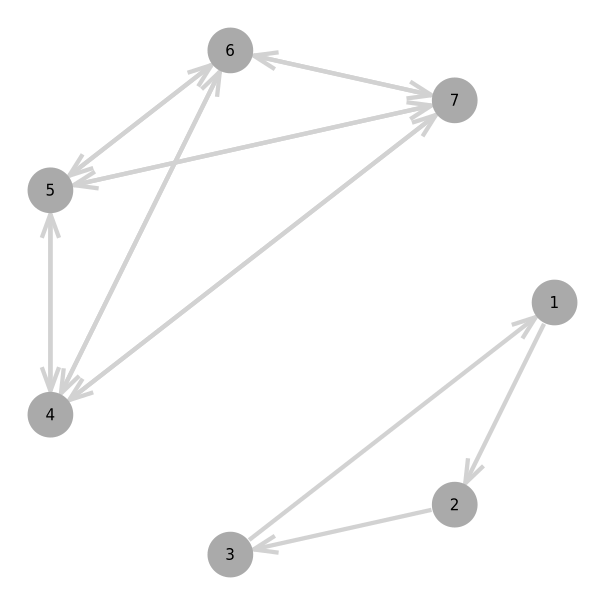
\includegraphics[width=0.42\textwidth]{img/triangle-tetrahedron.png}}
\caption*{Triangle with its tetrahedron complement $v_{123} + \star v_{123}$ in $\mb R^7$}
\end{figure}
John Browne has discussed Grassmann duality principle in book \cite{browne}, stating that every theorem (involving either of the exterior and regressive products) can be translated into its dual theorem by replacing the $\wedge$ and $\vee$ operations and applying \textit{Poincare duality} (homology).
First applying this Grassmann duality principle to the $\wedge$ product alone, let $\set{\omega_k}_k\in\Lambda^{p_k}V, P=\sum_kp_k$, then it is possible to obtain the co-product
$\bigvee :\Lambda^{p_1}V_1\times\dots\times\Lambda^{p_g}V_g \ra \Lambda^{P-(g-1)\#V}\bigcup_k V_k$.
Grassmann's original notation implicitly combined $\wedge,\vee,\star$.
The join $\wedge$ product is analogous to union $\cup$, the meet $\vee$ product is analogous to intersection $\cap$, and the orthogonal complement $\star\mapsto^\perp$ is negation.
Together, $(\wedge,\vee,\star)$ yield an orthocomplementary propositional lattice (quantum logic):
\begin{align*}
	(\star\bigvee_k &\omega_k)(v_1,\dots,v_P) = (\bigwedge_k\star\omega_k)(v_1,\dots,v_P) \quad \textit{DeMorgan's Law},
\end{align*}
where DeMorgan's law is used to derive tensor contractions.
\begin{definition}
	Skew left $\lrcorner$ and right $\llcorner$ contractions are symmetrically defined
	$ \gen{\omega}_r\cdot\gen{\eta}_s = \begin{cases} \omega\llcorner\eta=\omega\vee\star\eta & r\geq s \\ \omega\lrcorner\eta=\eta\vee\star\omega & r\leq s \end{cases} $.
	Note for $\omega,\eta$ of equal grade, $\omega\circledast\eta = \omega\odot\eta = \omega\cdot\eta = \omega\llcorner\eta = \omega\lrcorner\eta$ are all symmetric operations. In Julia, $\lrcorner$ is $<$ and $\llcorner$ is $>$.
\end{definition}

\begin{definition}
	Let $\nabla = \sum_k\partial_kv_k$ be a vector field and $\epsilon = \sum_k\epsilon_k(x)w_k \in \Omega^1V$ be unit sums of the mixed-symmetry basis.
	Elements of $\Omega^pV$ are known as \textit{differential} $p$-\textit{forms} and both $\nabla$ and $\epsilon$ are \textit{tensor fields} dependent on $x\in W$.
	Another notation for a differential form is $dx_k = \epsilon_k(x)w_k$, such that $\epsilon_k = dx_k/w_k$ and $\partial_k\omega(x) = \omega'(x)$.
\end{definition}
\begin{remark}
	The space $W$ does not have to equal $V\in\text{Vect}_{\mb K}$ above, as $\Omega^pV$ could have coefficients from $\mb K = LW$.
\end{remark}

\begin{definition}
	Define differential $d:\Omega^p V\ra\Omega^{p+1}V$ and co-differential $\delta:\Omega^pV\ra\Omega^{p-1}V$ such that \cite{bishop-goldberg}
	\begin{align*}
		\star d\omega &= \star(\nabla\wedge\omega) = \nabla\times\omega, & \omega\cdot\nabla &= \omega\vee\star\nabla = \partial\omega =-\delta\omega.
	\end{align*}
	These two maps have the special properties $d\circ d=0$ and $\partial\circ\partial = 0$ for any form $\omega$ and vector field $\nabla$. 
	In topology there is \textit{boundary} operator $\partial$ defined by $\partial\epsilon = \epsilon\cdot\nabla = \sum_k\partial_k\epsilon_k$ and is commonly discussed in terms the limit $\epsilon(x)\cdot\nabla\omega(x) = \lim_{h\ra0} \frac{\omega(x+h\epsilon)-\omega(x)}{h}$, which is the directional derivative \cite{sobczyk}.
\end{definition}
\begin{example}
	[Vorticity curl of vector-field]
	$\star d(dx_1+dx_2+dx_3) = (∂_2 -∂_3)dx_1 + (∂_3 -∂_1)dx_2 + (∂_1 -∂_2)dx_3$.
\end{example}
\begin{example}
	[Boundary of 3-simplex]
	Faces of simplex (oriented): $\partial(w_{1234}) = -\partial_4w_{123}+\partial_3w_{124}-\partial_2w_{134}+\partial_1w_{234}$.
\end{example}

\begin{theorem}[Integration by parts \& Stokes]
	Let $ \nabla \in\Omega_1 V $ be a Leibnizian vector field operator, then $d,-\partial$ are Hilbert adjoint Hodge-DeRahm operators with $\gen{\,\ast\,}$
	\begin{align*}
		\int_M d\omega\wedge\star\eta +\int_M \omega\wedge\star\partial\eta &= 0, & \gen{d\omega\ast\eta} &=\gen{\omega\ast-\partial\eta}.
	\end{align*}
\end{theorem}
\begin{proof}
	$\partial\omega = \omega\cdot\nabla = \star\inv(\star\omega\wedge\star^2\nabla) = (-1)^n(-1)^{nk}\star d\star\omega$.


	Then  substitute this into $\int_M \omega\wedge(-1)^{mk+m+1}\star\star d\star\eta = (-1)^{km+m+1}(-1)^{(m-k+1)(k-1)}\int_M\omega\wedge d\star\eta$,
	apply the identity $(-1)^{km+m+1}(-1)^{(m-k+1)(k-1)}=(-1)^k$ and
	$ (-1)^k\int_M\omega\wedge d\star\eta = \int_M d(\omega\wedge\star\eta) - (-1)^{k-1}\omega\wedge d\star\eta = \int_M d\omega\wedge\star\eta$.
	Stokes identity can be proved by relying on a variant of the \textit{common factor theorem} by Browne \cite{browne}.
\end{proof}
\begin{theorem}[Clifford-Dirac-Laplacian]
	The Dirac operator \cite{garling} is $ (\nabla^2)^\frac12\omega = \pm\nabla\ominus\omega = \pm\nabla\wedge\omega \pm \nabla\cdot\omega  = \pm d\omega\pm\partial\omega$.
	\begin{align*}
		\nabla^2\omega &= \nabla\wedge(\omega\cdot\nabla) + (\nabla\wedge\omega)\cdot\nabla) = \mp(\mp\omega\ominus\nabla)\ominus\nabla).
	\end{align*}
	Elements $\omega$ are \textit{harmonic} if $\nabla\omega = 0$ and both \textit{exact} $d\omega=0$ and \textit{coexact} $\delta\omega=0$, such that $\mc H^p M = \setc{\nabla\omega = 0}{\omega\in \Omega^pM}$.
	Hodge \cite{ivancevic}:
	$\Omega^pM=\mc H^pM\oplus\im{d\Omega^{p-1}M}\oplus\im{\partial\Omega^{p+1}M}$.
	Note: $\nabla\omega=-\omega\nabla, \nabla^2\omega=\omega\nabla^2$ for higher-order tensor fields!
\end{theorem}

\iffalse
\begin{lstlisting}[language = Julia]
julia> using Reduce, Grassmann; @basis tangent(ℝ^2,3,2);

julia> x = :x*v1 + ∂1v1 + ∂1*∂1v1 + ∂1*∂1*∂1v1
0.0 + xv₁ + (1 + (1 + 1∂₁)∂₁)∂₁v₁

julia> x^8
x ^ 8 + (8 * x ^ 7 + (4 * (2x + 7) * x ^ 6 + (8 * (x ^ 2 + 7x + 7) * x ^ 5)∂₁)∂₁)∂₁
\end{lstlisting}
\fi

%\subsection{Projective null-cones of Dirac-Clifford-Hestenes}

For the null-basis, complement operations are different:
\begin{align*}
	\star v_\infty &= \star(v_++v_-) = (v_- + v_+)v_{1...n} = v_{\infty1...n} \\
 	\star 2v_\emptyset &= \star(v_--v_+) = (v_+ - v_-)v_{1...n} = -2v_{\emptyset1...n}
\end{align*}
The Hodge complement satisfies $\gen{\omega\ast\omega}I=\omega\wedge\star\omega$. This property is naturally a result of using the geometric product in the definition.
An additional metric independent version of the complement operation is available with the \verb`!` operator,
\begin{align*}
	!v_\infty &= !(v_++v_-) = (v_- - v_+)v_{1...n} = 2v_{\emptyset1...n} \\
 	!2v_\emptyset &= !(v_--v_+) = (v_+ + v_-)v_{1...n} = -v_{\infty1...n}
\end{align*}
For that variation of complement, $||\omega||^2 I = \omega\,\wedge\,!\omega$ holds.
\begin{example}%[\textit{using Leibniz $\bigoplus\,$Grassmann}]
	S"$\infty\emptyset\text{+++"}(\nabla$\verb`^`$2) \,\,  \mapsto\, \, -2\partial_{\infty\emptyset} + \partial_1^2 + \partial_2^2 + \partial_3^2 $
\end{example}
Let $\nabla\in\Lambda^1V$, then $\omega = (\nabla\bs\nabla)\ominus\omega = \nabla\bs(d\omega + \partial\omega)$ where $\nabla\parallel\partial\omega$ and $\nabla\perp d\omega$.
Let's reflect across the hyperplane $\star\nabla$,
\begin{align*}
	\nabla\bs (d\omega-\partial\omega) &= \nabla\bs(d\omega-\partial\omega)\ominus(\nabla\bs\nabla) \\
									   &= -\nabla^2\bs(d\omega+\partial\omega)\ominus\nabla = -\nabla\bs\omega\ominus\nabla. %= \omega\oslash\nabla
\end{align*}
Hence, reflection by hyperplane $\star\nabla$ has isometry $\omega\oslash\nabla$ which for $\nabla = v_j$ is the map $\mb R^n \ra \mb R_1\times\cdots\times\conj{\mb R}_j\cdots\times\mb R_n$.

\begin{theorem}[Cartan-Dieudonne]
	Every isometry of $V\ra V$ is the composite of at most $k$ reflections across non-singular hyperplanes. Hence there exist vectors $\nabla_j$ such that
	$$ (((\omega\oslash\nabla_1)\oslash\nabla_2)\oslash\cdots)\oslash\nabla_k = \omega\oslash(\nabla_1\ominus\nabla_2\ominus\dots\ominus\nabla_k) $$
	for any isometry element of the orthogonal group $O(p,q)$.
\end{theorem}
Note that elements under transformations of this group preserve inner product relations.
The even grade operators make up the rotational group, where each bivector isometry is a composition of two reflections \cite{artin} \cite{doran-hestenes-sommen-acker}.

Consider the differential equation $ \partial_i\epsilon_j = \epsilon_j\oslash\omega$ with the solution $\epsilon_j(x) = \epsilon_j(0)\oslash e^{x_i\omega} $ where $\theta =2 x_i$ is the parameter of the Lie group. Then for a normalized $\omega$,
$$ e^{\theta\omega} = \sum_k \frac{(\theta\omega)^{\ominus k}}{k!} = \begin{cases} \cosh\theta+\omega\sinh\theta, & \text{if } \omega^2 = 1, \\ \cos\theta + \omega\sin\theta, & \text{if } \omega^2=-1, \\ 1+\theta\omega, & \text{if } \omega^2=0. \end{cases} $$
Note that $\nabla\oslash e^{\theta\omega/2} = \nabla \ominus e^{\theta\omega}$ is a double covering when using the complex numbers in the Euclidean plane.
\begin{theorem}[Leibniz-Taylor series]
	$\partial_X=\bigominus_k\partial_k^{\mu_k}$ is defined so that $|X|=\sum_k\mu_k$, then $e^{\partial\epsilon}\omega(x)$ is
	\begin{align*}
		e^{\partial\epsilon}\omega(x) =
		\sum_{j=0}^\mu \frac{(\partial\epsilon)^{\ominus j}}{j!}\omega(x)
		= \sum_{j=0}^\mu\sum_{|X|=j} \bigominus_k \frac{(\partial_{k}\epsilon_k(x))^{\mu_{k}}}{\mu_k!}\omega(x).
		%+ (\mu+1)\sum_{|X|=\mu+1}\int_0^1(1-t)^\mu\bigominus_k\frac{(\partial_k\epsilon_k(x))^{\mu_k}}{\mu_k!}\omega(x+t\epsilon)\,dt.
	\end{align*}
\end{theorem}
The multivariate \textit{product rule} is encoded into the geometric algebraic product when using mixed-symmetry.

\begin{lstlisting}[language = Julia]
using Grassmann, Makie
basis"2" # Euclidean
streamplot(vectorfield(exp(π*v12/2)),-1.5..1.5,-1.5..1.5)
streamplot(vectorfield(exp((π/2)*v12/2)),-1.5..1.5,-1.5..1.5)
streamplot(vectorfield(exp((π/4)*v12/2)),-1.5..1.5,-1.5..1.5)
streamplot(vectorfield(v1*exp((π/4)*v12/2)),-1.5..1.5,-1.5..1.5)
@basis S"+-" # Hyperbolic
streamplot(vectorfield(exp((π/8)*v12/2)),-1.5..1.5,-1.5..1.5)
streamplot(vectorfield(v1*exp((π/4)*v12/2)),-1.5..1.5,-1.5..1.5)
\end{lstlisting}
\begin{figure}[ht]
	\centering
	%\caption{Euclidean vector fields based on exponential operator:}
	\begin{subfigure}[b]{0.23\textwidth}
		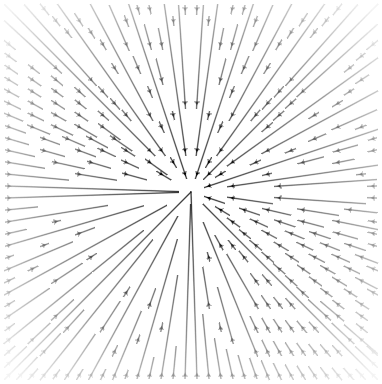
\includegraphics[width=\textwidth]{img/plane-1.png}
		\caption{$x\oslash e^{\pi v_{12}/2}$, $\mb R^2$}
		%\label{fig:sample_figure}
	\end{subfigure}
	~
	\begin{subfigure}[b]{0.23\textwidth}
		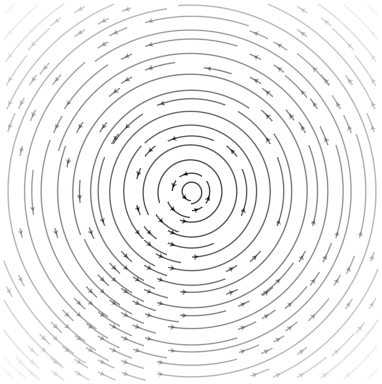
\includegraphics[width=\textwidth]{img/plane-2.png}
		\caption{$ x\oslash e^{\frac\pi2 v_{12}/2}$, $\mb R^2$}
		%\label{fig:sample_figure}
	\end{subfigure}
	
	\begin{subfigure}[b]{0.23\textwidth}
		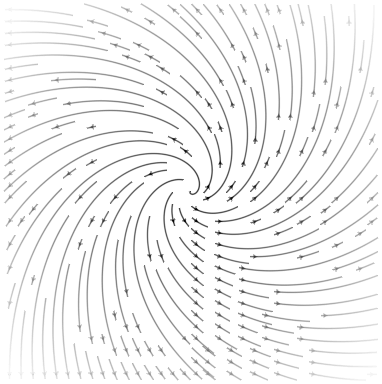
\includegraphics[width=\textwidth]{img/plane-3.png}
		\caption{$x\oslash e^{\frac\pi4 v_{12}/2}$, $\mb R^2$}
		%\label{fig:sample_figure}
	\end{subfigure}
	~
	\begin{subfigure}[b]{0.23\textwidth}
		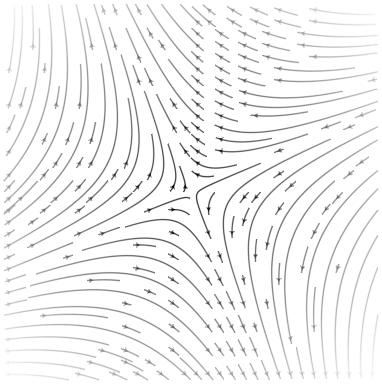
\includegraphics[width=\textwidth]{img/plane-4.png}
		\caption{$x\oslash(v_1\ominus e^{\frac\pi4 v_{12}/2})$, $\conj{\mb R}\oplus\mb R$}
		%\label{fig:sample_figure}
	\end{subfigure}

	\begin{subfigure}[b]{0.23\textwidth}
		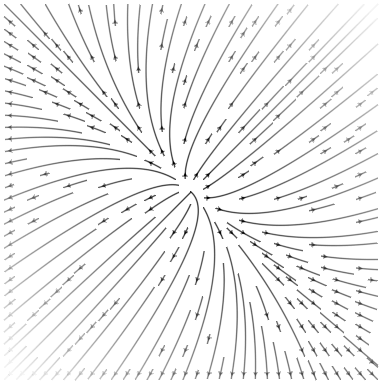
\includegraphics[width=\textwidth]{img/plane-5.png}
		\caption{$x\oslash e^{\frac\pi8 v_{12}/2}$, $\mb R\oplus\mb R'$}
		%\label{fig:sample_figure}
	\end{subfigure}
	~
	\begin{subfigure}[b]{0.23\textwidth}
		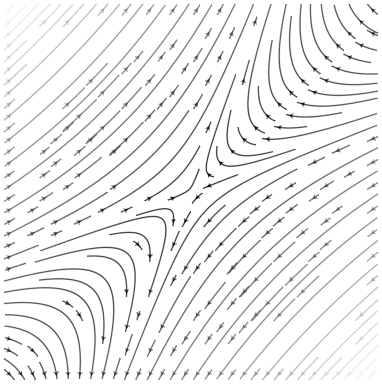
\includegraphics[width=\textwidth]{img/plane-6.png}
		\caption{$x\oslash(v_1\ominus e^{\frac\pi4 v_{12}/2})$, $\conj{\mb R}\oplus\mb R'$}
		%\label{fig:sample_figure}
	\end{subfigure}
\end{figure}

As a result of Grassmann's exterior \& interior products, the Hodge-DeRahm chain complex from cohomology theory is
\begin{align*}
	0 &\os d{\us\partial\rightleftarrows} \Omega^0(M) \os d{\us\partial\rightleftarrows} \Omega^1(M) \os d{\us\partial\leftrightarrows} \cdots \os d{\us\partial\rightleftarrows} \Omega^n(M) \os d{\us\partial\rightleftarrows} 0,
\end{align*}
having dimensional equivalence brought by the Grassmann-Poincare-Hodge complement duality,
\begin{align*}
	\mc H^{n-p}M &\cong \frac{\ker(d\Omega^{n-p}M)}{\im{d\Omega^{n-p+1}M}}, & \dim\mc H^pM &= \dim\frac{\ker(\partial\Omega^pM)}{\im{\partial\Omega^{p+1}M}}
\end{align*}
The rank of the grade $p$ boundary incidence operator is
$$ \text{rank}\gen{\partial\gen{M}_{p+1}}_p = \min\set{\dim\gen{\partial\gen{M}_{p+1}}_p,\dim\gen{M}_{p+1}} $$
Invariant topological information can be computed using the rank of homology groups, where $b_p(M)=\dim\mc H^pM$ are
$$ b_p(M) = \dim\gen{M}_{p+1} - \text{rank}\gen{\partial\gen{M}_{p+1}}_p - \text{rank}\gen{\partial\gen{M}_{p+2}}_{p+1} $$
Betti numbers with Euler characteristic $\chi(M) = \sum_p (-1)^pb_p$.

Let's obtain the full \verb`skeleton` of a simplical complex $\Delta(\omega)=\mc P(\omega)\bs\Lambda^0(V)$ from the power set $\mc P(\omega)$ of all vertices with each \verb`subcomplex` $\Delta(\partial(\omega))$ contained in the edge graph:
$$ \Delta(\omega) =  \sum_{g=1}^n\sum_{k=1}^{n\choose g}\plr{\text{abs}\gen{\omega}_{g,k} + \Delta\plr{\text{abs}\,\partial\gen{\omega}_{g,k}}}. $$
\begin{example}
	[Topology] Compute the value $\chi(\Delta(\omega))=1$ and $\chi(\Delta(\partial(\omega))) = \, ?$ for any \verb`Simplex` $\omega$. As an exercise, also compute the corresponding \verb`betti` numbers..
\end{example}

In Fig. 4, different possible discrete bivector topologies in a projective Riemann sphere setting are examined. 
The figures are based on the product topology of two rotation bivectors.
When the Euclidean $\mb R^4$ basis is combined with projective geometric algebra, resulting one parameter Lie groups can be visualized as a fibration of a torus in $\mb R^3$. 
When the fourth $v_\infty$ basis direction is rotated into the Minkowski plane, the double rotation becomes a helix with translational single rotation. In examples (b)$\sim$(c) the bivector is modulated.

\begin{figure}[t]
	\centering
	\caption{Variations of sub-manifold vector field mappings in $\mb R^4$.}
	\begin{subfigure}[b]{0.23\textwidth}
		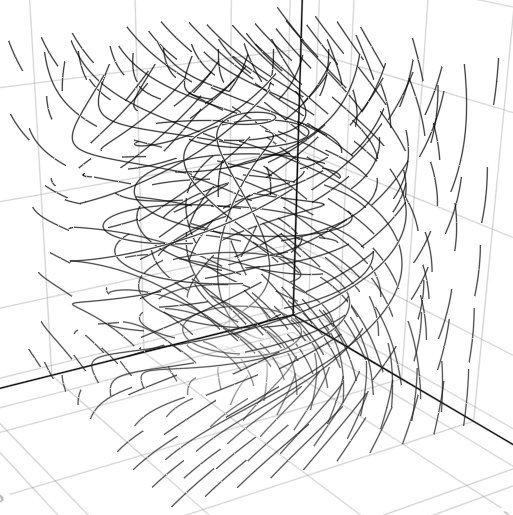
\includegraphics[width=\textwidth]{img/orb.png}
		\caption{$x\oslash e^{\frac\pi4(v_{12}+v_{\infty3})}$}
		%\label{fig:sample_figure}
	\end{subfigure}
	~
	\begin{subfigure}[b]{0.23\textwidth}
		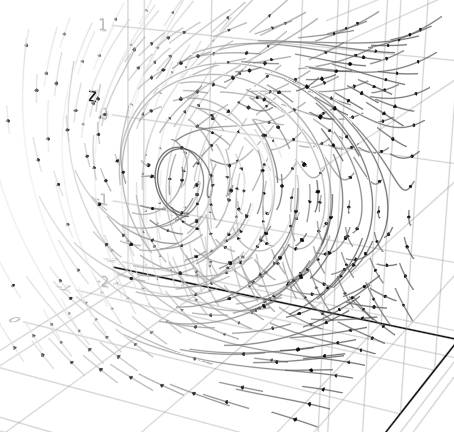
\includegraphics[width=\textwidth]{img/wave.png}
		\caption{$V_{\infty12}\ra V_{123}$}
		%\label{fig:sample_figure}
	\end{subfigure}
\end{figure}

\section{Conclusion}

\textit{Grassmann.jl} and its accompanying support packages provide an extensible platform for fully generalized computing with geometric algebra at high dimensions.
%This will enable the usage of many different types of \verb`TensorAlgebra` along with various \verb`VectorBundle` parameters and interoperability for a wide range of scientific and research applications.
All of the types and operations in this paper are implemented using only a few thousand lines of code with Julia's type polymorphism code generation, with the mixed-symmetry interaction of \verb`Leibniz` and \verb`Grassmann` available for research.
%The goal is to algebraically define operator actions on groups of \textit{Leibniz.jl} differential function elements. 
%One way is to use \textit{Reduce.jl} for differentiation and \textit{SyntaxTree.jl} to obtain optimal symbolic polynomial forms \cite{optim-poly}.
Thus, computations involving fully general rotational algebras and Lie bivector groups are possible with a full trigonometric suite. % enabled by $ e^{A} = \sum_n \frac{A^n}{n!} $.
Conformal geometric algebra is possible with the Minkowski plane $v_{\infty\emptyset}$, based on the null-basis.
In general, multivalued quantum logic is enabled by the $\wedge,\vee,\star$ Grassmann lattice.
Mixed-symmetry algebra with \textit{Leibniz.jl} and \textit{Grassmann.jl}, having the geometric algebraic product chain rule, yields automatic differentiation and Hodge-DeRahm co/homology  as unveiled by Grassmann.
Most importantly, the Dirac-Clifford product yields generalized Hodge-Laplacian and the Betti numbers with Euler characteristic \verb`χ`.

\textbf{Acknowledgements}: Many thanks for discussions with Steven De Keninck, Utensil Song, Alexander Arsenovic, Hugo Hadfield, Karl Wessel; the helpful Julia community (e.g. Jameson Nash, Stefan Karpinski, Jeff Bezanson, Kristoffer Carlsson, Petr Krysl, Nathan Smith, Hongying Li, etc); and thanks for support from my family.

%\cite{bezanson2017julia}

\begin{figure}[t]
	\centering
	\caption{Different variations of bivectors in $\mb R^4$ discrete topology.}
	\begin{subfigure}[b]{0.14\textwidth}
		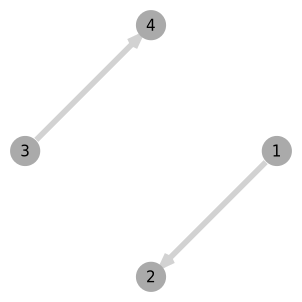
\includegraphics[width=\textwidth]{img/graph-1.png}
		\caption{$v_{12}+v_{34}$}
		%\label{fig:sample_figure}
	\end{subfigure}
	~
	\begin{subfigure}[b]{0.14\textwidth}
		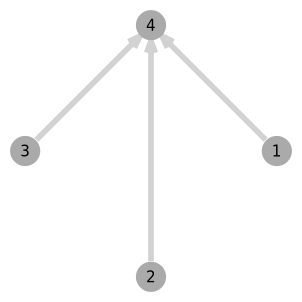
\includegraphics[width=\textwidth]{img/graph-2.png}
		\caption{$v_{14}+v_{24}+v_{34}$}
		%\label{fig:sample_figure}
	\end{subfigure}
	~
	\begin{subfigure}[b]{0.14\textwidth}
		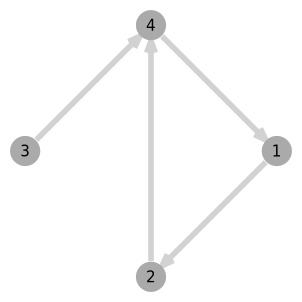
\includegraphics[width=\textwidth]{img/graph-3.png}
		\caption{$\partial v_{124}+v_{34}$}
		%\label{fig:sample_figure}
	\end{subfigure}
\end{figure}

\begin{figure}[ht]
	\centering
	%\caption{Doubly-periodic flow from independent bivectors:}
	\begin{subfigure}[b]{0.3\textwidth}
		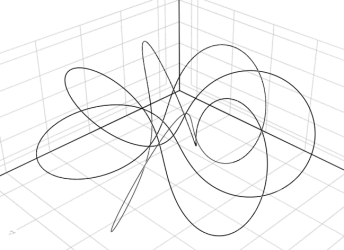
\includegraphics[width=\textwidth]{img/torus.png}
		\caption{Doubly periodic flow (independent)}
		%\label{fig:sample_figure}
	\end{subfigure}
	~
	\begin{subfigure}[b]{0.15\textwidth}
		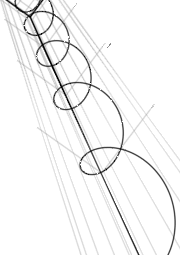
\includegraphics[width=\textwidth]{img/helix.png}
		\caption*{(a) Period translation}
		%\label{fig:sample_figure}
	\end{subfigure}
\end{figure}

\begin{figure}[ht]
	\begin{subfigure}[b]{0.16\textwidth}
		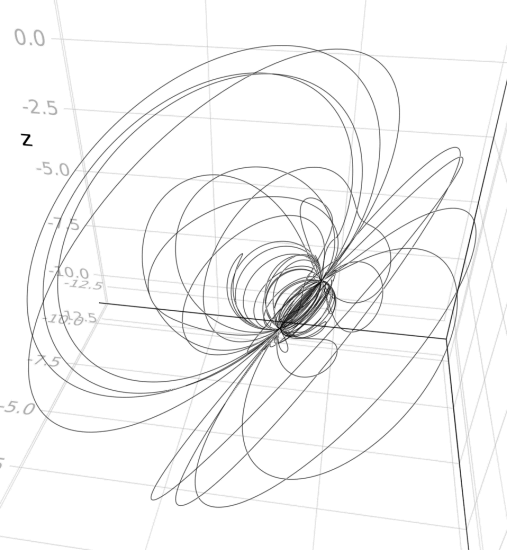
\includegraphics[width=\textwidth]{img/orbit-2.png}
		%\caption{$x\oslash e^{\pi v_{12}/2}$}
		%\label{fig:sample_figure}
	\end{subfigure}
	~
	\begin{subfigure}[b]{0.28\textwidth}
		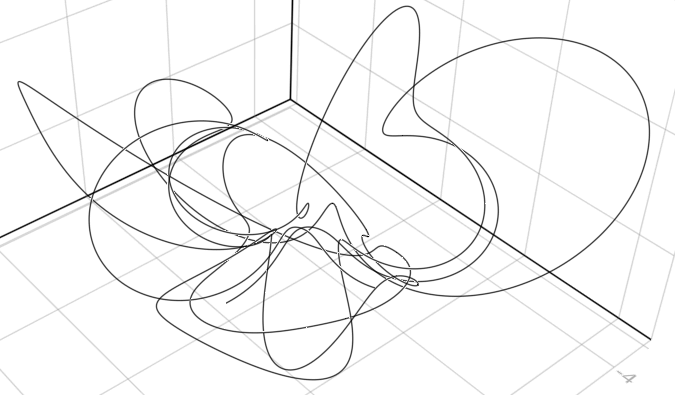
\includegraphics[width=\textwidth]{img/orbit-4.png}
		%\caption{$ x\oslash e^{\frac\pi2 v_{12}/2}$}
		%\label{fig:sample_figure}
	\end{subfigure}
	\caption*{(b)$\sim$(c) $\downarrow(e^{tv_\infty(sin(3t)3v_1+cos(2t)7v_2-sin(5t)4v_3)/2}\obackslash\uparrow(v_1+v_2-v_3))$}
\end{figure}

% **************GENERATED FILE, DO NOT EDIT**************

\bibliographystyle{juliacon}
\bibliography{ref.bib}


\end{document}
